\section{Questions}

In this section we look at question 1 subquestion a, 
we want to add this extra explanation bla bla, and also 
note bla bla. \\

Out script is given by:
\lstinputlisting{Hand-In-1.py}

The printed results of the script are:

\lstinputlisting{Hand-In-1.txt}

Our script produces the following plots.

\begin{figure}[h!]
  \centering
  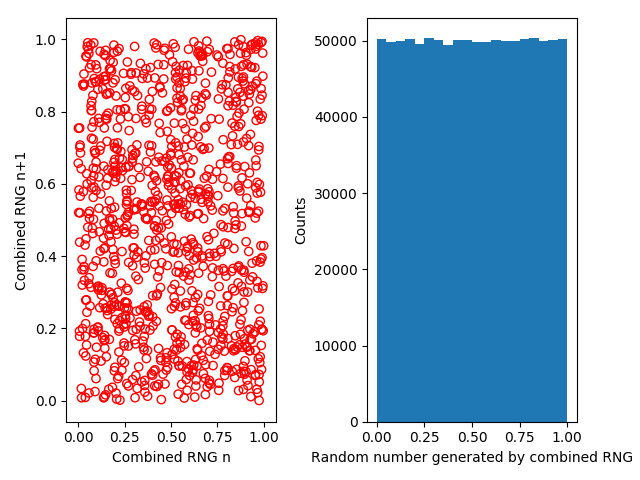
\includegraphics[width=0.9\linewidth]{./plots/RNG-test-results.png}
  \caption{Solution to Question 1b}
  \label{fig:fig1}
\end{figure}

\begin{figure}[h!]
  \centering
  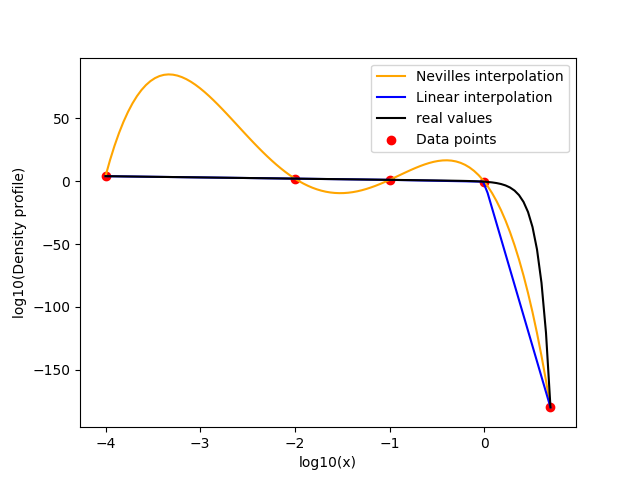
\includegraphics[width=0.9\linewidth]{./plots/Log-Log_plot_interpolation.png}
  \caption{Literature result, say something...}
  \label{fig:fig2}
\end{figure}

\begin{figure}[h!]
  \centering
  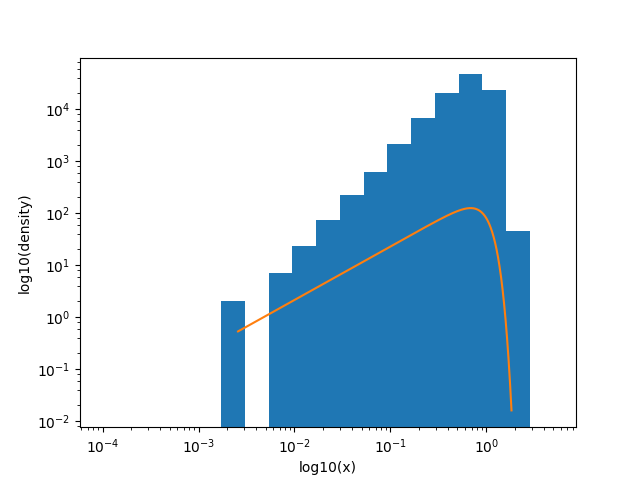
\includegraphics[width=0.9\linewidth]{./plots/Density_profile_Haloes_Log-Log2.png}
  \caption{Literature result, say something...}
  \label{fig:fig3}
\end{figure}

\begin{figure}[h!]
  \centering
  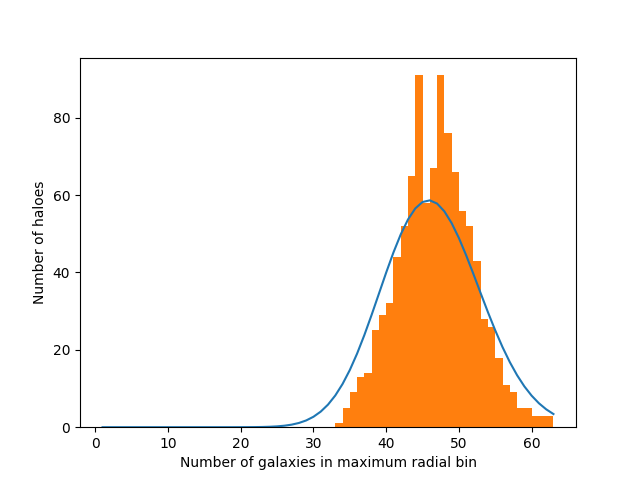
\includegraphics[width=0.9\linewidth]{./plots/Counts_of_bins.png}
  \caption{Literature result, say something...}
  \label{fig:fig4}
\end{figure}

\begin{figure}[h!]
  \centering
  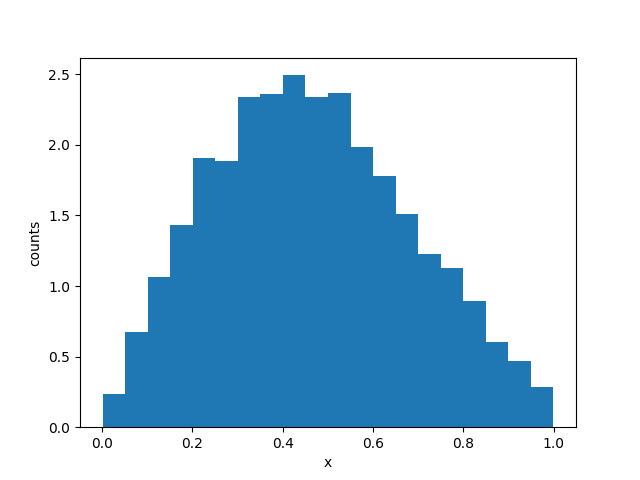
\includegraphics[width=0.9\linewidth]{./plots/Densityprofile_readin_gal.png}
  \caption{Literature result, say something...}
  \label{fig:fig5}
\end{figure}
